\chapter{Экспериментальная часть}
Используя расчетную программу построенную на базе приведенной выше математической модели, было проведено моделирование нормального падения моноэнергетического пучка электронов на подложку с нанесенным на неё слоем резиста. Энергия электронов задана на уровне 20 кэВ, подложка выполнена из кремния толщиной 5000 нм, а резист выполнен из ПММА и имел толщину 500 нм.

\begin{figure}[h]
    \center
    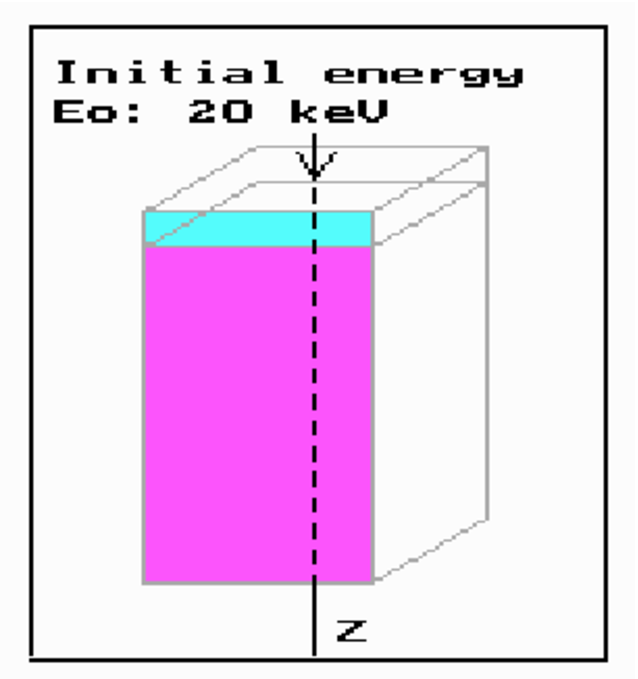
\includegraphics[width=.47\textwidth]{example}
    \caption{Схематическое изображение подложки с нанесенным на нее резистом}
    \label{fig:example}
\end{figure}

В налетающем пучке распределение плотноси энергии имеет вид, представленный на рисунке~\ref{fig:beam}.
\begin{figure}[h]
    \center
    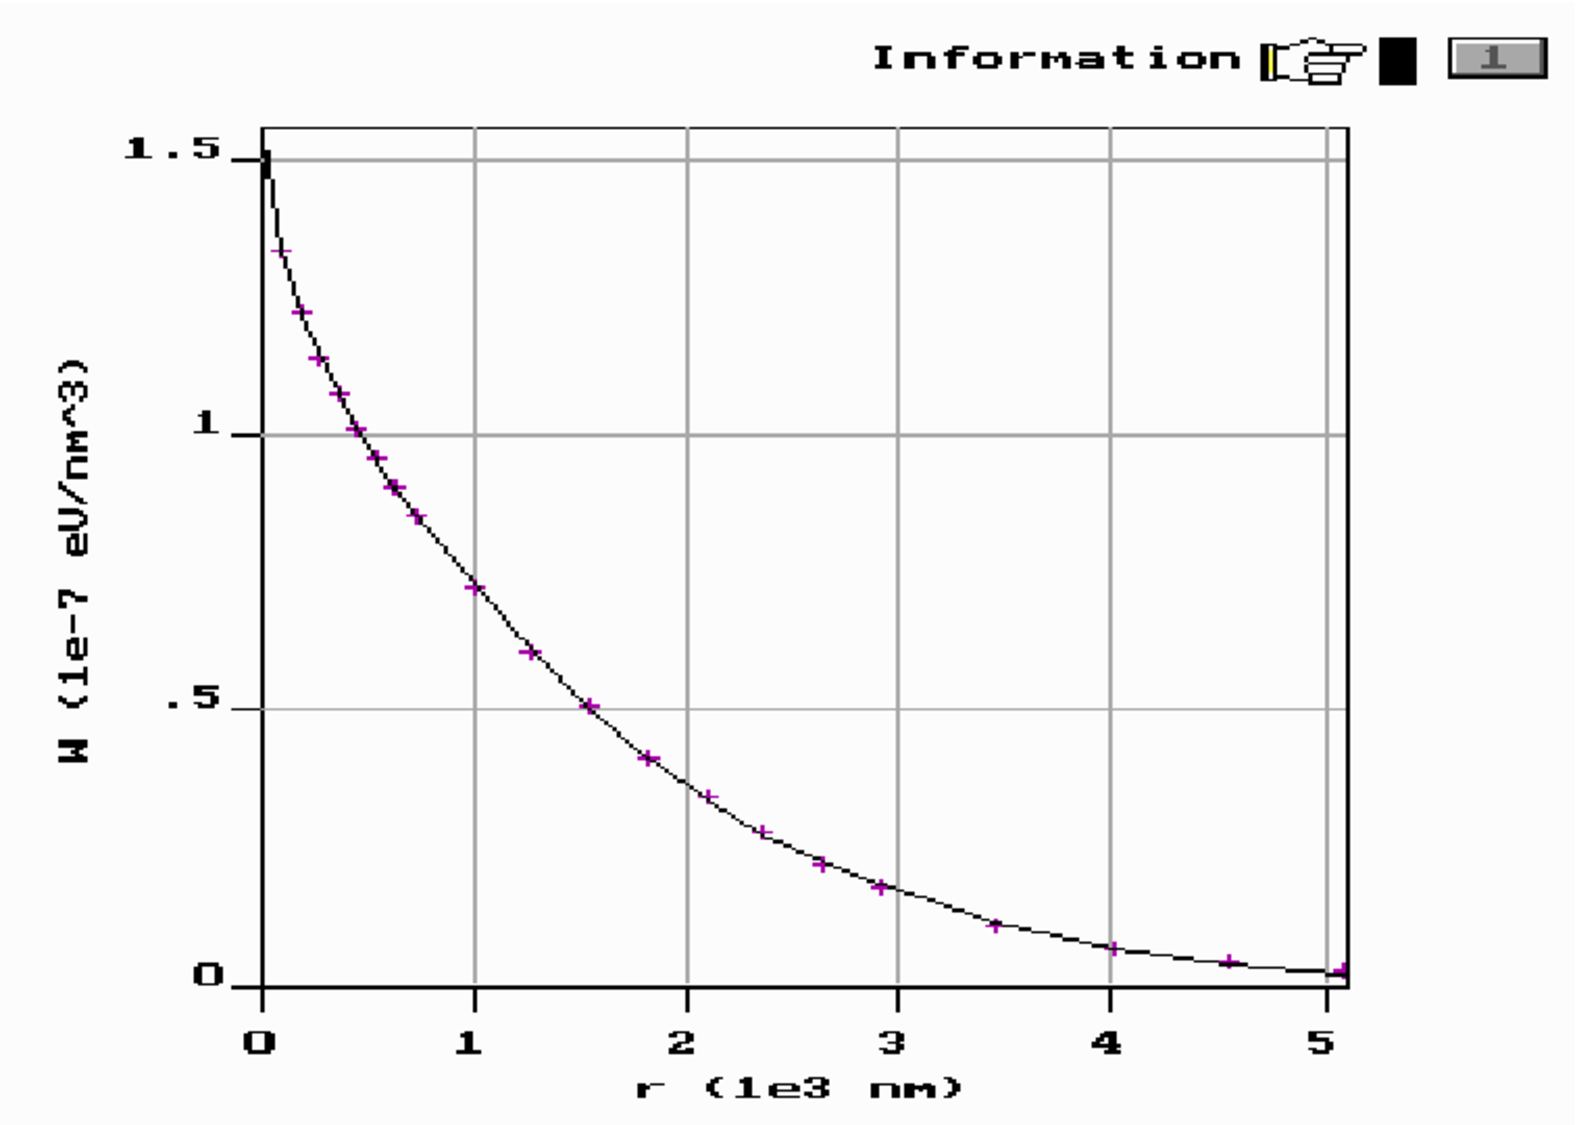
\includegraphics[width=.95\textwidth]{beam}
    \caption{радиальное распределение плотности энергии в налетающем пучке}
    \label{fig:beam}
\end{figure}

Как можно видеть из графика, представленного на рис.~\ref{fig:fluxes}, при данном значении энергии лишь малая часть электронов отражается обратно, в основном они диффундируют. Что говорит о малом количестве эелектронов учавствующих в эффекте близости.
% здесь можно приплести про эффект близости
\begin{figure}[h]
    \center
    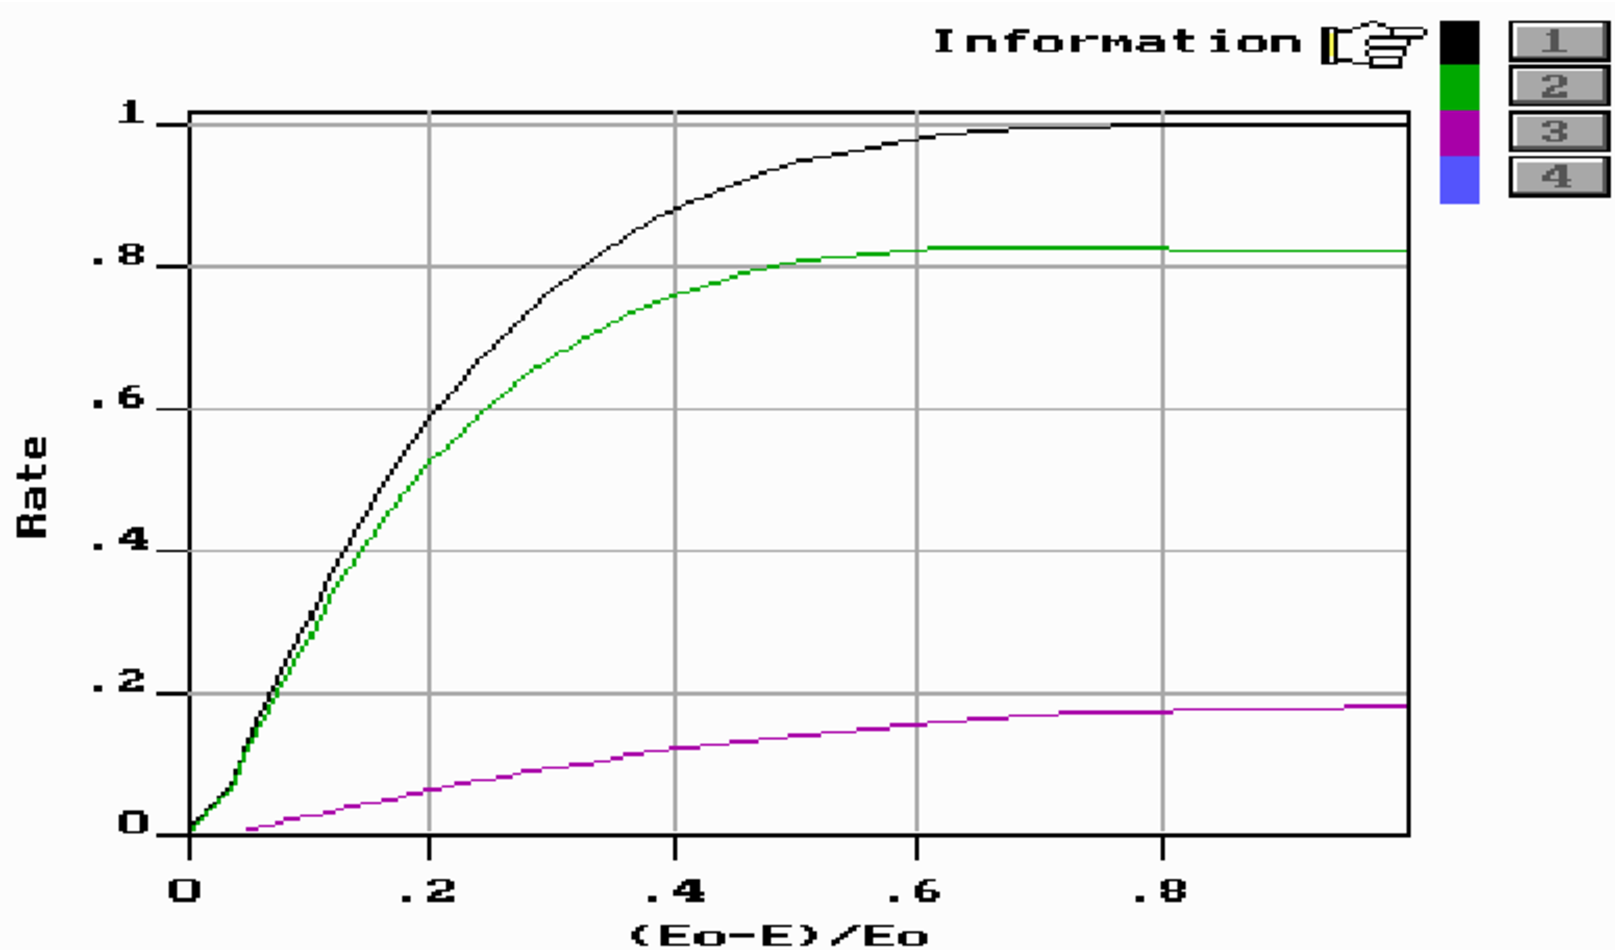
\includegraphics[width=.95\textwidth]{fluxes}
    \caption{Доля потоков электронов:
    1 -- электроны, перешедшие из налетающих в диффузионные;
2 -- дифундировавшие электроны с энергией $E$;
3 -- отраженные электроны с энергие от $E_0$ до $E$;
4 -- прошедшие насквозь через подложку электроны с энергией от $E_0$ до $E$.
}
    \label{fig:fluxes}
\end{figure}


По мере прохождения доля диффузионных электронов растёт.

\begin{figure}[h]
    \center
    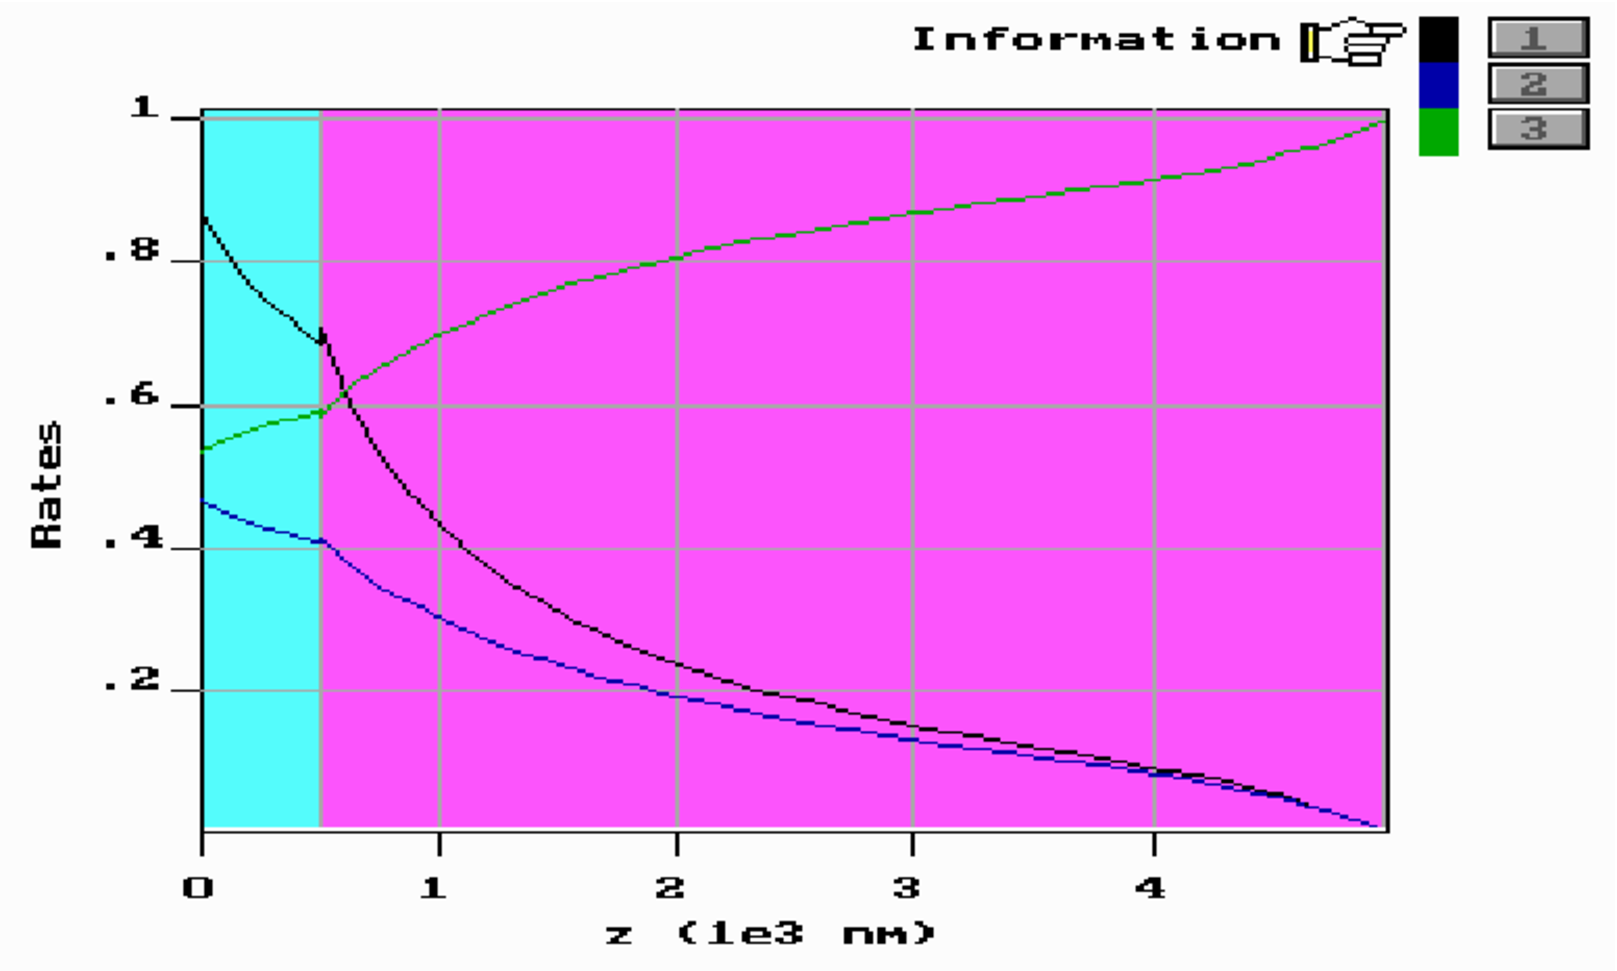
\includegraphics[width=.95\textwidth]{rates}
    \caption{Соотношение диффузионных и нерассеянных электронов: 1 -- отношение потока нерассеянных электронов к потоку диффузионных;
2 -- доля потока нерассеянных электронов;
3 -- доля потока диффузионных электронов.
}
    \label{fig:rates}
\end{figure}

При прохождении в глубь резиста, а впоследствии и подложки, пучок уширяется
\begin{figure}[h]
    \center
    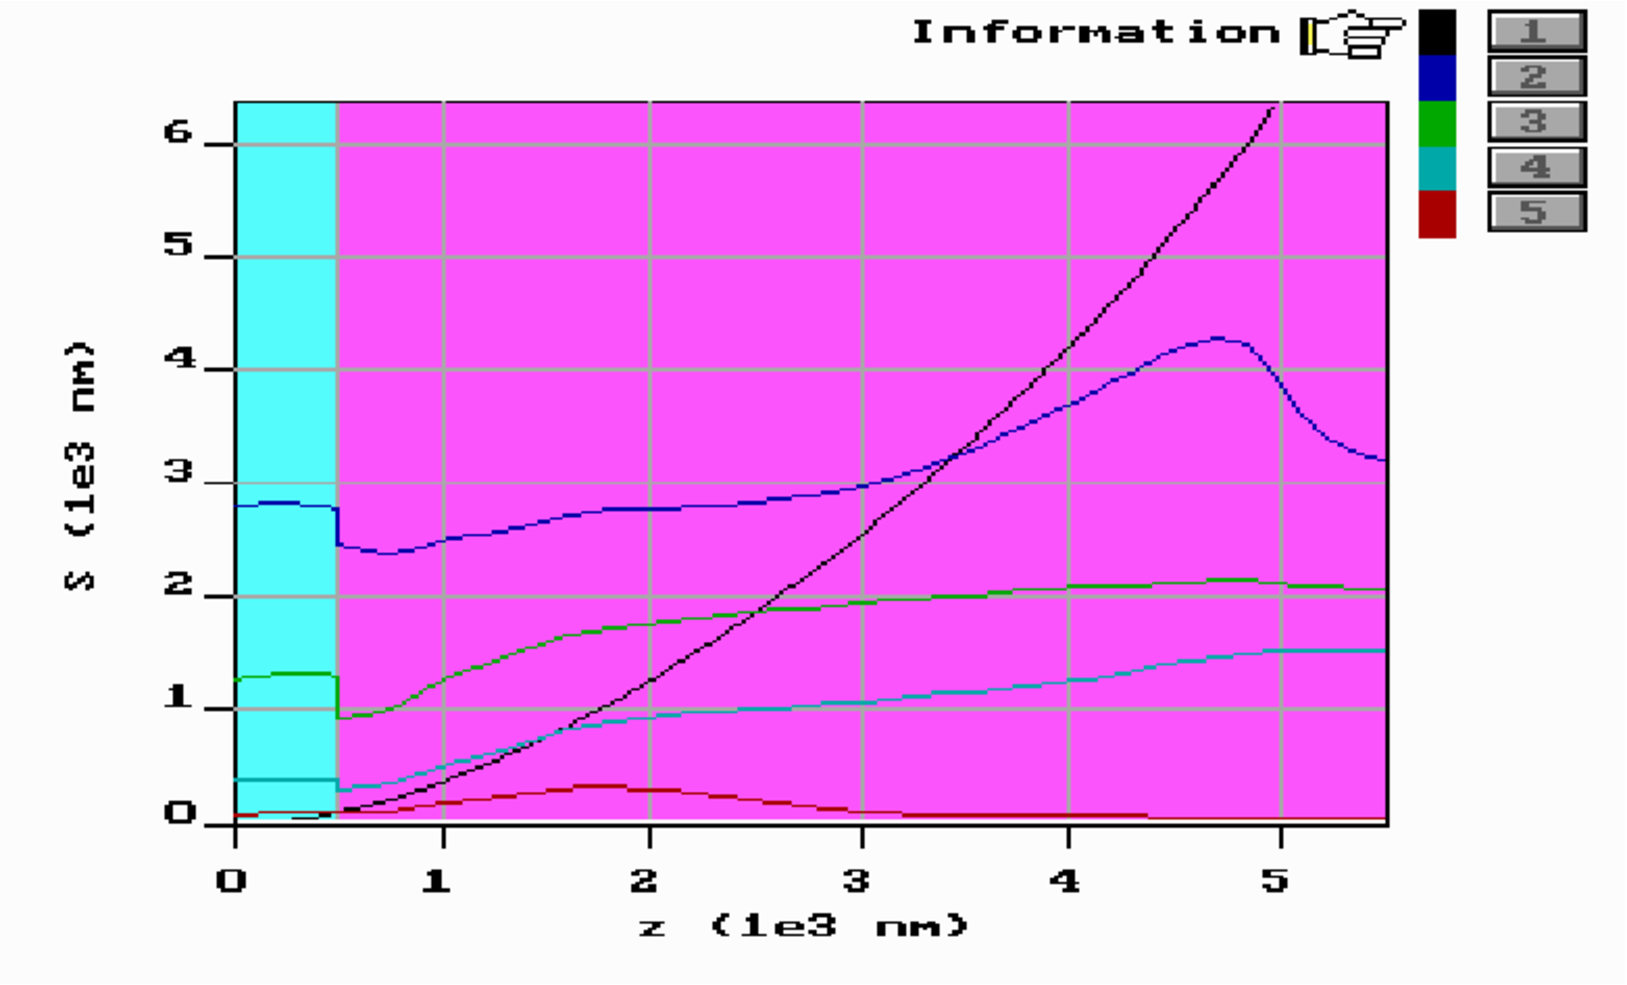
\includegraphics[width=.95\textwidth]{sequence}
    \caption{Поперечные размеры пучка:
1 -- полуширина пучка нерассеянных электронов;
2 -- полуширина пучка диффувзионных электронов по 1-му гауссиану;
3 -- полуширина пучка диффувзионных электронов по 2-му гауссиану;
4 -- полуширина пучка диффувзионных электронов по 3-му гауссиану;
5 -- полуширина пучка диффувзионных электронов по 4-му гауссиану.}
    \label{fig:sequence}
\end{figure}


\begin{figure}[h]
    \center
    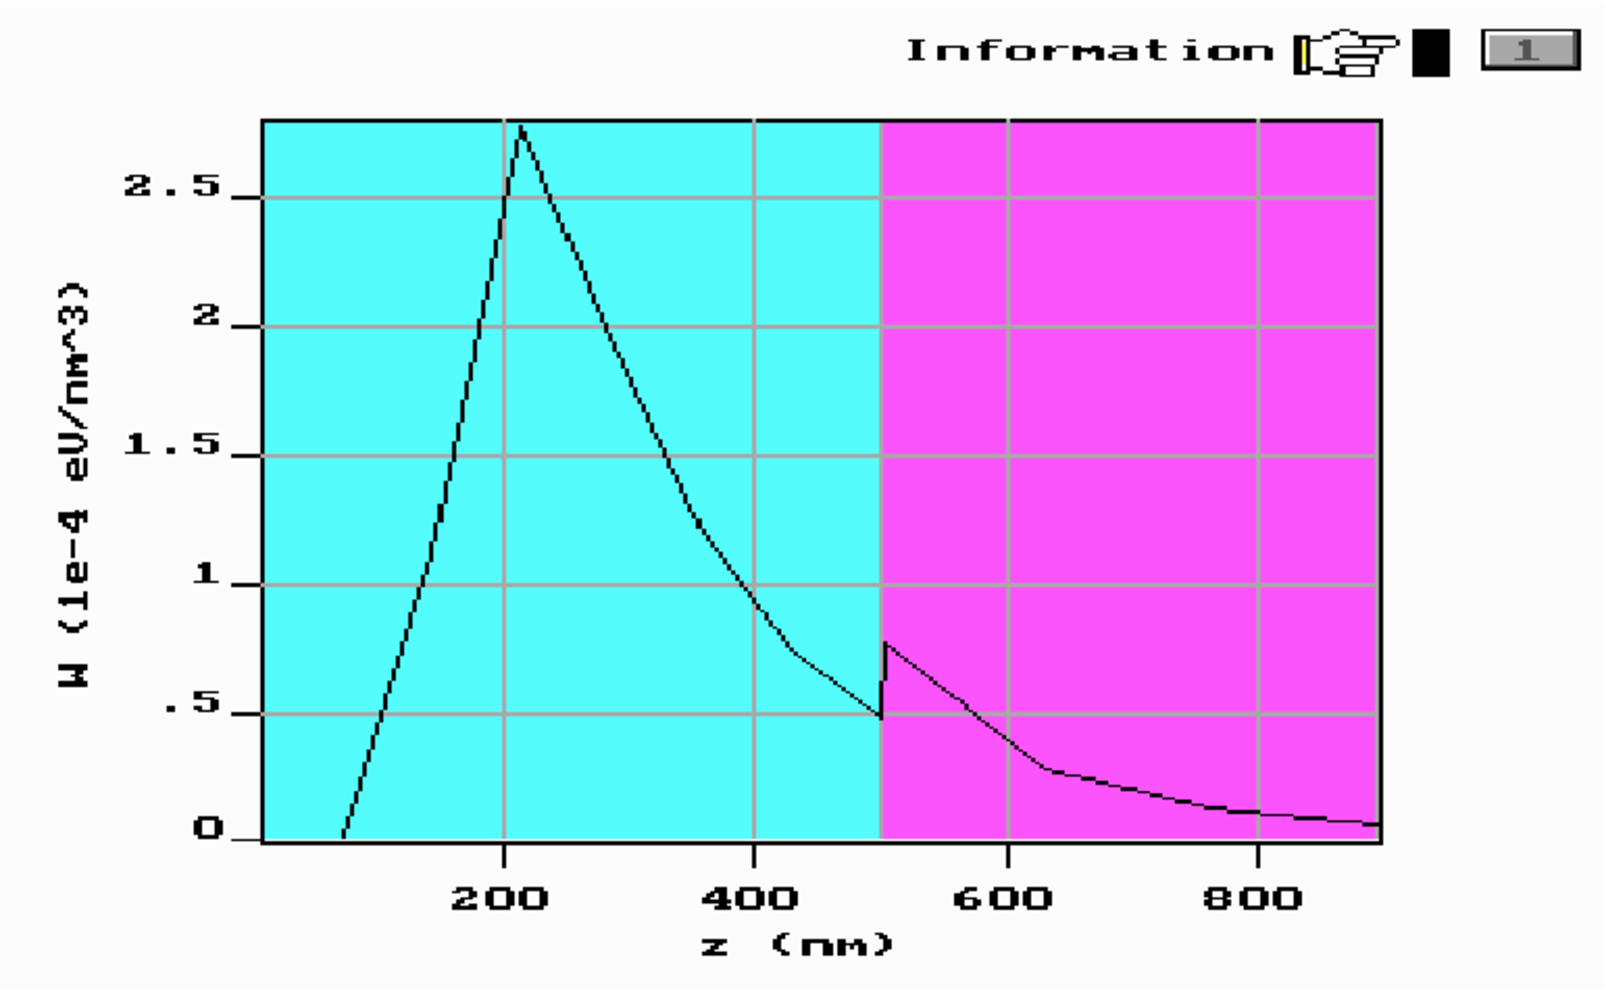
\includegraphics[width=.95\textwidth]{absorption}
    \caption{Зависимость от глубины плотности поглощенной энергии нерассеянных электрорнов в расчете на 1 электрон 1 для пучка радиусом 24.3 нм}
    \label{fig:absorption}
\end{figure}

Из зависимости показанной на рис.~\ref{fig:sequence} видно что пр прохождении пучка через резист на глубине пути примерно 230 нм, находится максимум поглощения энергии пучка резистом и мишенью в целом. Следующий максимум поглощения находится в приграничной зоне подлжки и резиста, далее интенсивность спадает. Данные результаты можно интерпритировать слдеующим образом. Пи использовании относительно изкой энерги электронного пучка при прохождении его через резист он начинает диффундировать, и в последствии поглащаться резистом, так как энергии электронов относительно не велеки. При переходе в подложку, те электроны которые прошли через резист 2 на рис.~\ref{fig:fluxes} и не были поглощены но потеряли энергию в результате диффузии, при переходе в более плотную среду, поглащаются.






можно сделать вывод что , при пр



